
\section{Аймаг сумдын мэдээлэл авдаг форм}

Уг формыг хийж гүйцэтгэж React-н анхан шатны туршлагатай болох зорилготой байсан ба цаашид ажилласан төсөл дээр хэрэглэж буй зарим сан болох Material-ui, react-select-н ажиллагааг ойлгох, тодорхой хэмжээнд практик мэдлэгийг цуглуулж чадсан. 

Сурах ур чадвар: 
\begin{itemize}
    \item Асуудлаа тодорхойлж бага багаар шийдвэрлэх чадварт суралцах
    \item Git ашиглаж, бичсэн кодоо хадгалах
    \item Шинэ технологиудыг өөрийн бичсэн код дээрээ хэрэгжүүлэх
\end{itemize}

Формын шаардлага: 
\begin{itemize}
    \item Next.js ашигласан байна
    \item Functional component ашиглаж, тухайн component-н дотоод төлвийг ашиглах
    \item Эцэг сонголтыг өөрчлөхөд хүү сонголтуудын утга цэвэрлэгддэг байх
    \item useEffect hook ашиглах
    \item Дараагийн шатанд форм дээрээ Material-ui нэвтрүүлэх
    \item Дараагийн шатанд useReducer ашигласан байх
    \item Дараагийн шатанд react-select санг нэвтрүүлэх
\end{itemize}

\begin{figure}
    \centering
    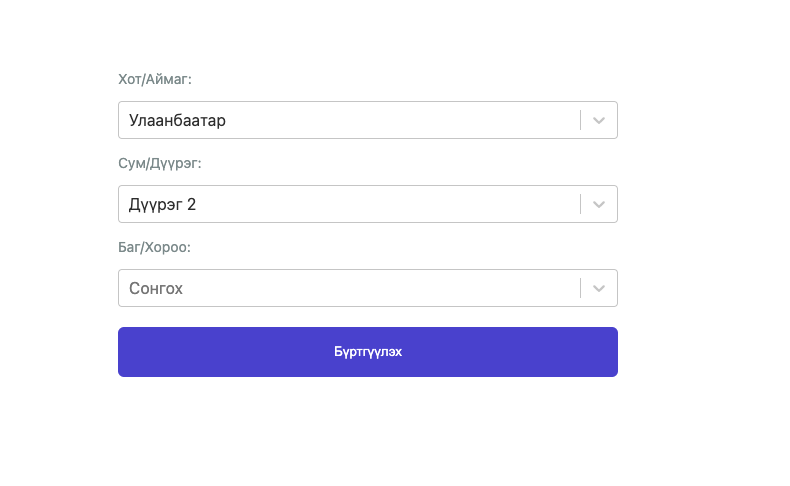
\includegraphics[width=15cm]{images/form.png}
    \caption{Формын эцсийн байдлаар харагдаж буй байдал}
    \label{fig:my_label}
\end{figure}
\subsection{useEffect болон useState ашиглан формын мэдээллийг шаардлагын дагуу авах}

Эхний ээлжинд ямар нэгэн загваргүй зөвхөн формын зөв ажиллагаа буюу логик үйлдлүүд дээр анхаарах хэрэгтэй байсан ба хамгийн түрүүнд хийх шаардлагатай зүйл нь аймаг сумдын датаг next.js дээрээ үүсгэсэн api-аасаа авч дэлгэцэнд харуулах байсан юм. 

\begin{lstlisting}[language=Javascript, caption=Next.js дээр бичсэн серверээс датагаа татаж авах, frame=single]
const fetchData = (url) => {
  return axios
    .get(`http://localhost:3000/api/${url}`)
    .then((res) => {
      const results = res.data;
      return results;
    })
    .catch((err) => {
      console.error(err);
    });
};
\end{lstlisting}

Доор харагдаж буй хэсэгт компонентийн логик үйлдлүүд харагдаж байна. useForm() hook ашиглаж select-н утга өөрчлөгдсөн эсэхийг барьж авах, functional component ашиглан state дотор хэрэглэгчийн сонгосон аймаг, сум, хороог хадгална. 

\begin{lstlisting}[language=Javascript, caption=Component-н үндсэн логик үйлдлүүд, frame=single]
export default function Home() {
  const [values, handleChange] = useForm();
  const [data, setData] = useState({
    cities: [],
    districts: [],
    wards: [],
  });

  useEffect(() => {
    fetchData(`cities`)
      .then((res) => {
        setData({ ...data, cities: res });
      })
      .catch((err) => {
        console.error(err);
      });
  }, []);

  const register = (e) => {
    e.preventDefault();
    console.log(values);
  };

  const handleSelect = (id, type) => {
    if (type == "city") {
      fetchData(`cities/${id}`)
        .then((res) => {
          setData({ ...data, districts: res, wards: [] }); //set districts and clear wards data
        })
        .catch((err) => {
          console.error(err);
        });
    } else if (type == "district") {
      //get wards
      fetchData(`cities/${values.city}/${id}`)
        .then((res) => {
          setData({ ...data, wards: res });
        })
        .catch((err) => {
          console.error(err);
        });
    }
  };
  
  ...
\end{lstlisting}
